\documentclass[11pt, a4paper]{article}

\usepackage[a4paper, margin=2.2cm]{geometry}
\usepackage[utf8]{inputenc}
\usepackage[T1]{fontenc}
% Magyar nyelv: a babel saját hungarian nyelvi beállítása (babel-hu.ini).
% A [magyar] opció helyett ez kell, mert a telepített magyar.ldf újabb a babel csomagnál,
% és a kettő együtt nem fordul le. Ez is magyar elválasztást, „Tartalomjegyzék”-et és „ábra” feliratot ad.
\usepackage{babel}
\babelprovide[import, main]{hungarian}
\usepackage{lmodern}
\usepackage{enumitem}
\setlist[itemize]{label=-}
\usepackage{booktabs}
\usepackage{graphicx} % Hozzáadva a nagyméretű UML ábrák szélességének auto-skálázásához
\usepackage{tikz} % Az állapotgép-ábrához
\usetikzlibrary{shapes.multipart, positioning, arrows.meta} % Az UML-ábrához
\usepackage[colorlinks=true, linkcolor=black, urlcolor=blue]{hyperref}
% A hosszú \texttt neveket nem lehet elválasztani; inkább kicsit nagyobb legyen a szóköz, mint hogy kilógjanak a margóra
\setlength{\emergencystretch}{3em}

% Magyar tipográfia: a fejezetszám után pont áll („1. A feladat”), az ábrafelirat „1. ábra” alakú
\makeatletter
\renewcommand{\@seccntformat}[1]{\csname the#1\endcsname.\quad}
\renewcommand{\fnum@figure}{\thefigure.~\figurename}
\makeatother

\usepackage{fancyhdr}
\pagestyle{fancy}
\fancyhf{}
\lhead{\textbf{PAC-MAN}}
\rhead{Tari Balázs}
\cfoot{\thepage}
\renewcommand{\headrulewidth}{0.4pt}

\begin{document}

\begin{titlepage}
    \centering
    \vspace*{4cm}
    {\Huge \textbf{PAC-MAN} \par}
    \vspace{1.5cm}
    {\LARGE A programozás alapjai 3. \par}
    \vspace{0.5cm}
    {\Large Feladatspecifikáció \par}
    \vspace{4.5cm}
    {\Large \textbf{Tari Balázs} \par}
    \vspace{0.3cm}
    {\Large E3K6W5 \par}
    \vfill
    {\large 2026. november \par}
\end{titlepage}

\tableofcontents
\newpage
\sloppy

% --- 1. A feladat ---
\section{A feladat}
A Pac-Man egy kétdimenziós arcade játék. A játékos a sárga figurát irányítja egy labirintusban: össze kell gyűjtenie az összes pöttyöt, és közben el kell kerülnie a négy szellemet, amelyek mindegyike másképp üldözi őt. A labirintusban négy power pellet is van; ha Pac-Man megeszik egyet, a szellemek egy ideig megijednek, és ilyenkor ő eheti meg őket további pontokért. Ha egy szellem elkapja, Pac-Man életet veszít; három élet után a játéknak vége. Ha minden pötty elfogyott, ugyanaz a pálya újraindul a következő szinten, ahol rövidebb ideig tart a szellemek ijedtsége.

A program Java Swing grafikus felületen fut. A játék bármikor elmenthető és később folytatható, a befejezett játékok pontszáma ranglistára kerül, és egy beépített pályaszerkesztővel saját pályák is rajzolhatók. A játékmodellt automatizált JUnit 5 egységtesztek ellenőrzik.

% --- 2. Használati esetek ---
\section{Használati esetek}
\begin{enumerate}[itemsep=2pt]
    \item \textbf{Új játék:} a főmenü \textit{Start new game} gombja fájlválasztót nyit a \texttt{maps} mappában (a beépített \texttt{level1.txt} van kijelölve). A kiválasztott pályán 0 ponttal, 3 élettel, az 1. szinten indul a játék. Irányítás: \texttt{W}/\texttt{A}/\texttt{S}/\texttt{D}.
    \item \textbf{Pontgyűjtés és szintlépés:} a megevett pötty és power pellet eltűnik, és pontot ér. Ha mind elfogyott, ugyanaz a labirintus jön újra a következő szinten; a pontszám és az életek megmaradnak.
    \item \textbf{Ütközés a szellemekkel:} egy üldöző szellem egy életbe kerül, egy ijedt szellemet Pac-Man megeszik. Nulla életnél \texttt{GAME OVER}.
    \item \textbf{Ranglista:} a játék végén a pontszám automatikusan, névbekérés nélkül bekerül a \texttt{highscores.csv}-be. A \textit{Leaderboard} képernyő a legjobbtól a leggyengébbig mutatja az eredményeket.
    \item \textbf{Mentés és folytatás:} a \textit{SAVE \& QUIT} gomb vagy az \texttt{F5} szünetelteti a játékot, egy párbeszédablakban bekéri a mentés nevét, ment, és visszalép a menübe. A \textit{Load previous game} bármelyik mentést pontosan ott folytatja, ahol abbamaradt.
    \item \textbf{Pályaszerkesztő:} a \textit{Create map} egy üres, $19 \times 21$ mezős rácsot nyit, rögzített szellemházzal. Egérrel falat, pöttyöt, power pelletet és Pac-Man kezdőmezőjét lehet rajzolni, majd a pályát a \texttt{maps} mappába menteni és rajta játszani.
\end{enumerate}

% --- 3. A megoldás vázlata ---
\section{A megoldás vázlata}
\textbf{Technológiák:} Java 17, Swing (\texttt{JFrame}, \texttt{JPanel}, \texttt{CardLayout} a képernyőváltáshoz, \texttt{JFileChooser}, \texttt{Graphics} az alacsony szintű rajzoláshoz, \texttt{javax.swing.Timer} a 60 tick/másodperces ciklushoz), a gyűjtemény-keretrendszer (\texttt{List}, \texttt{ArrayList}, \texttt{Comparator}), Java bináris szerializáció, szöveges fájlkezelés (\texttt{java.nio.file.Files}), JUnit 5.

\textbf{Fájlformátumok} (részletesen: \ref{sec:io}.~fejezet): \texttt{highscores.csv} (\texttt{PlayerName;Score;Date}), pályafájlok (a labirintus karakteres rajza), \texttt{.dat} mentések (szerializált \texttt{GameEngine}).

\textbf{Architektúra (MVC):} a modell (\texttt{hu.bme.pacman.game}) semmit sem tud a felületről: egyetlen osztálya sem importál Swinget vagy AWT-t. A felület és a fájlkezelés a \texttt{hu.bme.pacman.system} csomagban van, ide tartozik a belépési pont (\texttt{Main}) is, az enumok a \texttt{hu.bme.enums} csomagban.

\subsection*{A modell osztályai}
\begin{itemize}[itemsep=2pt]
    \item \textbf{\texttt{GameEngine}:} a játékszabályok. Tárolja a pontszámot, az életeket, a szintet, a labirintust, Pac-Mant és a szellemeket. Az \texttt{update()} egy tick, a \texttt{step()} egy mezőnyi lépés (\ref{sec:game_loop}.~fejezet). Létrehozáskor eltesz egy érintetlen másolatot a pályáról (\texttt{originalMap}), ebből állítja vissza a pöttyöket a \texttt{nextLevel()}. Mentés: \texttt{saveGameState(file)}; betöltés: a statikus \texttt{loadGameState(file)}, amely új motort ad vissza, mert az adattagok többsége \texttt{final}. Egy közös \texttt{Random}-ot használ, amelyet a tesztek rögzített seeddel adhatnak át.
    \item \textbf{\texttt{Labyrinth}:} \texttt{CellType[][]} rács, \texttt{grid[sor][oszlop]} indexeléssel. A rácson kívüli mező falnak számít, így semmi sem hagyhatja el a pályát. \texttt{isWalkable}, \texttt{isIntersection} (legalább 3 járható szomszéd), \texttt{hasDotsLeft}, valamint \texttt{copy()}: mély másolat, soronként \texttt{Arrays.copyOf}-fal, mert egy 2D tömb \texttt{clone()}-ja a sorokat megosztaná, és egy megevett pötty a másolatból is eltűnne.
    \item \textbf{\texttt{GameObject}} (absztrakt): mezőkoordináták (\texttt{x} = oszlop, \texttt{y} = sor), sebesség, irány, valamint a kezdőmező (\texttt{resetToStart()}) és az előző mező (\texttt{rememberPosition()}). Az előző mezőt a nézet a folyamatos rajzoláshoz, az ütközésvizsgálat a helycsere felismeréséhez használja.
    \item \textbf{\texttt{PacMan}:} a pufferelt billentyűparancsot tárolja (\texttt{currentCommand}, \texttt{transient}), és a \texttt{processInput()} futtatja le. A \texttt{resetToStart()} a pufferelt parancsot is eldobja.
    \item \textbf{\texttt{Ghost}:} állapot (\texttt{GhostState}), személyiség és stratégiaobjektum. A \texttt{possibleDirections()} a visszafordulás nélkül járható irányokat adja (zsákutcában a visszafordulást is); ebből választ a \texttt{chooseDirection()} véletlenszerűen és a \texttt{chooseDirectionTowards()} egy célmező felé. Az állapotváltásokat a \texttt{frighten()}, \texttt{calmDown()}, \texttt{eaten()}, \texttt{respawn()} végzi.
    \item \textbf{\texttt{GhostStrategy}} és megvalósításai, \textbf{\texttt{Tile}} (módosíthatatlan osztály a célmezőnek), \textbf{\texttt{Command}}/\textbf{\texttt{MoveCommand}}, \textbf{\texttt{LevelData}} (egy pályafájl tartalma: labirintus, Pac-Man, szellemek): lásd \ref{sec:design_patterns}.~fejezet.
\end{itemize}

\subsection*{A felület és a fájlkezelés osztályai}
\begin{itemize}[itemsep=2pt]
    \item \textbf{\texttt{MainFrame}:} a főablak; \texttt{CardLayout}-tal vált a menü, a játék, a ranglista és a szerkesztő között (\texttt{switchScreen}). Egyszerre csak egy játékpanel és egy szerkesztő létezik; kilépéskor a panelt leállítja és eltávolítja, mert egy rejtett panel \texttt{Timer}-e tovább futna.
    \item \textbf{\texttt{MainMenu}:} négy gomb (\texttt{startBtn}, \texttt{loadGameBtn}, \texttt{leaderboardBtn}, \texttt{editorBtn}). Ő tölti be a pályát vagy a mentést, így a játékpanel mindig kész \texttt{GameEngine}-t kap; hibás fájl esetén hibaüzenetet mutat.
    \item \textbf{\texttt{GamePanel}:} a játék képernyője. A \texttt{Timer}-e hajtja a játékot, a WASD billentyűket \texttt{MoveCommand}-dá alakítja, a \texttt{paintComponent} kirajzolja a világot és az állapotsort (pontszám, életek, szint, \textit{SAVE \& QUIT}). Játék végén pontosan egyszer írja be a pontszámot a ranglistába, a nevet a \texttt{System.getProperty("user.name")} adja.
    \item \textbf{\texttt{LeaderboardPanel}:} a ranglista csak olvasható nézete; minden megjelenítéskor újraolvassa a fájlt (\texttt{refresh()}).
    \item \textbf{\texttt{MapEditor}:} kattintható $19 \times 21$-es rács rögzített, zárolt szellemházzal és négy eszközzel (fal, pötty, power pellet, Pac-Man kezdőmezője). Bal egérgomb rajzol, jobb töröl, húzással is. Mentés előtt ellenőrzi, hogy van-e Pac-Man és legalább egy pötty; a \texttt{level1.txt} nem írható felül.
    \item \textbf{\texttt{LevelManager}:} állapot nélküli, statikus segédosztály (Factory): pályafájl $\leftrightarrow$ \texttt{LevelData} (\texttt{loadFromCSV}, \texttt{saveToCSV}), ranglista (\texttt{loadHighscores}, \texttt{appendHighscore}), valamint a fájl- és mappanevek. \textbf{\texttt{HighscoreEntry}:} a ranglista egy sora (módosíthatatlan adathordozó osztály).
\end{itemize}

\begin{figure}[p]
    \centering
    \resizebox{\textwidth}{!}{ % Ráhúzza a diagramot a maximális lapszélességre
    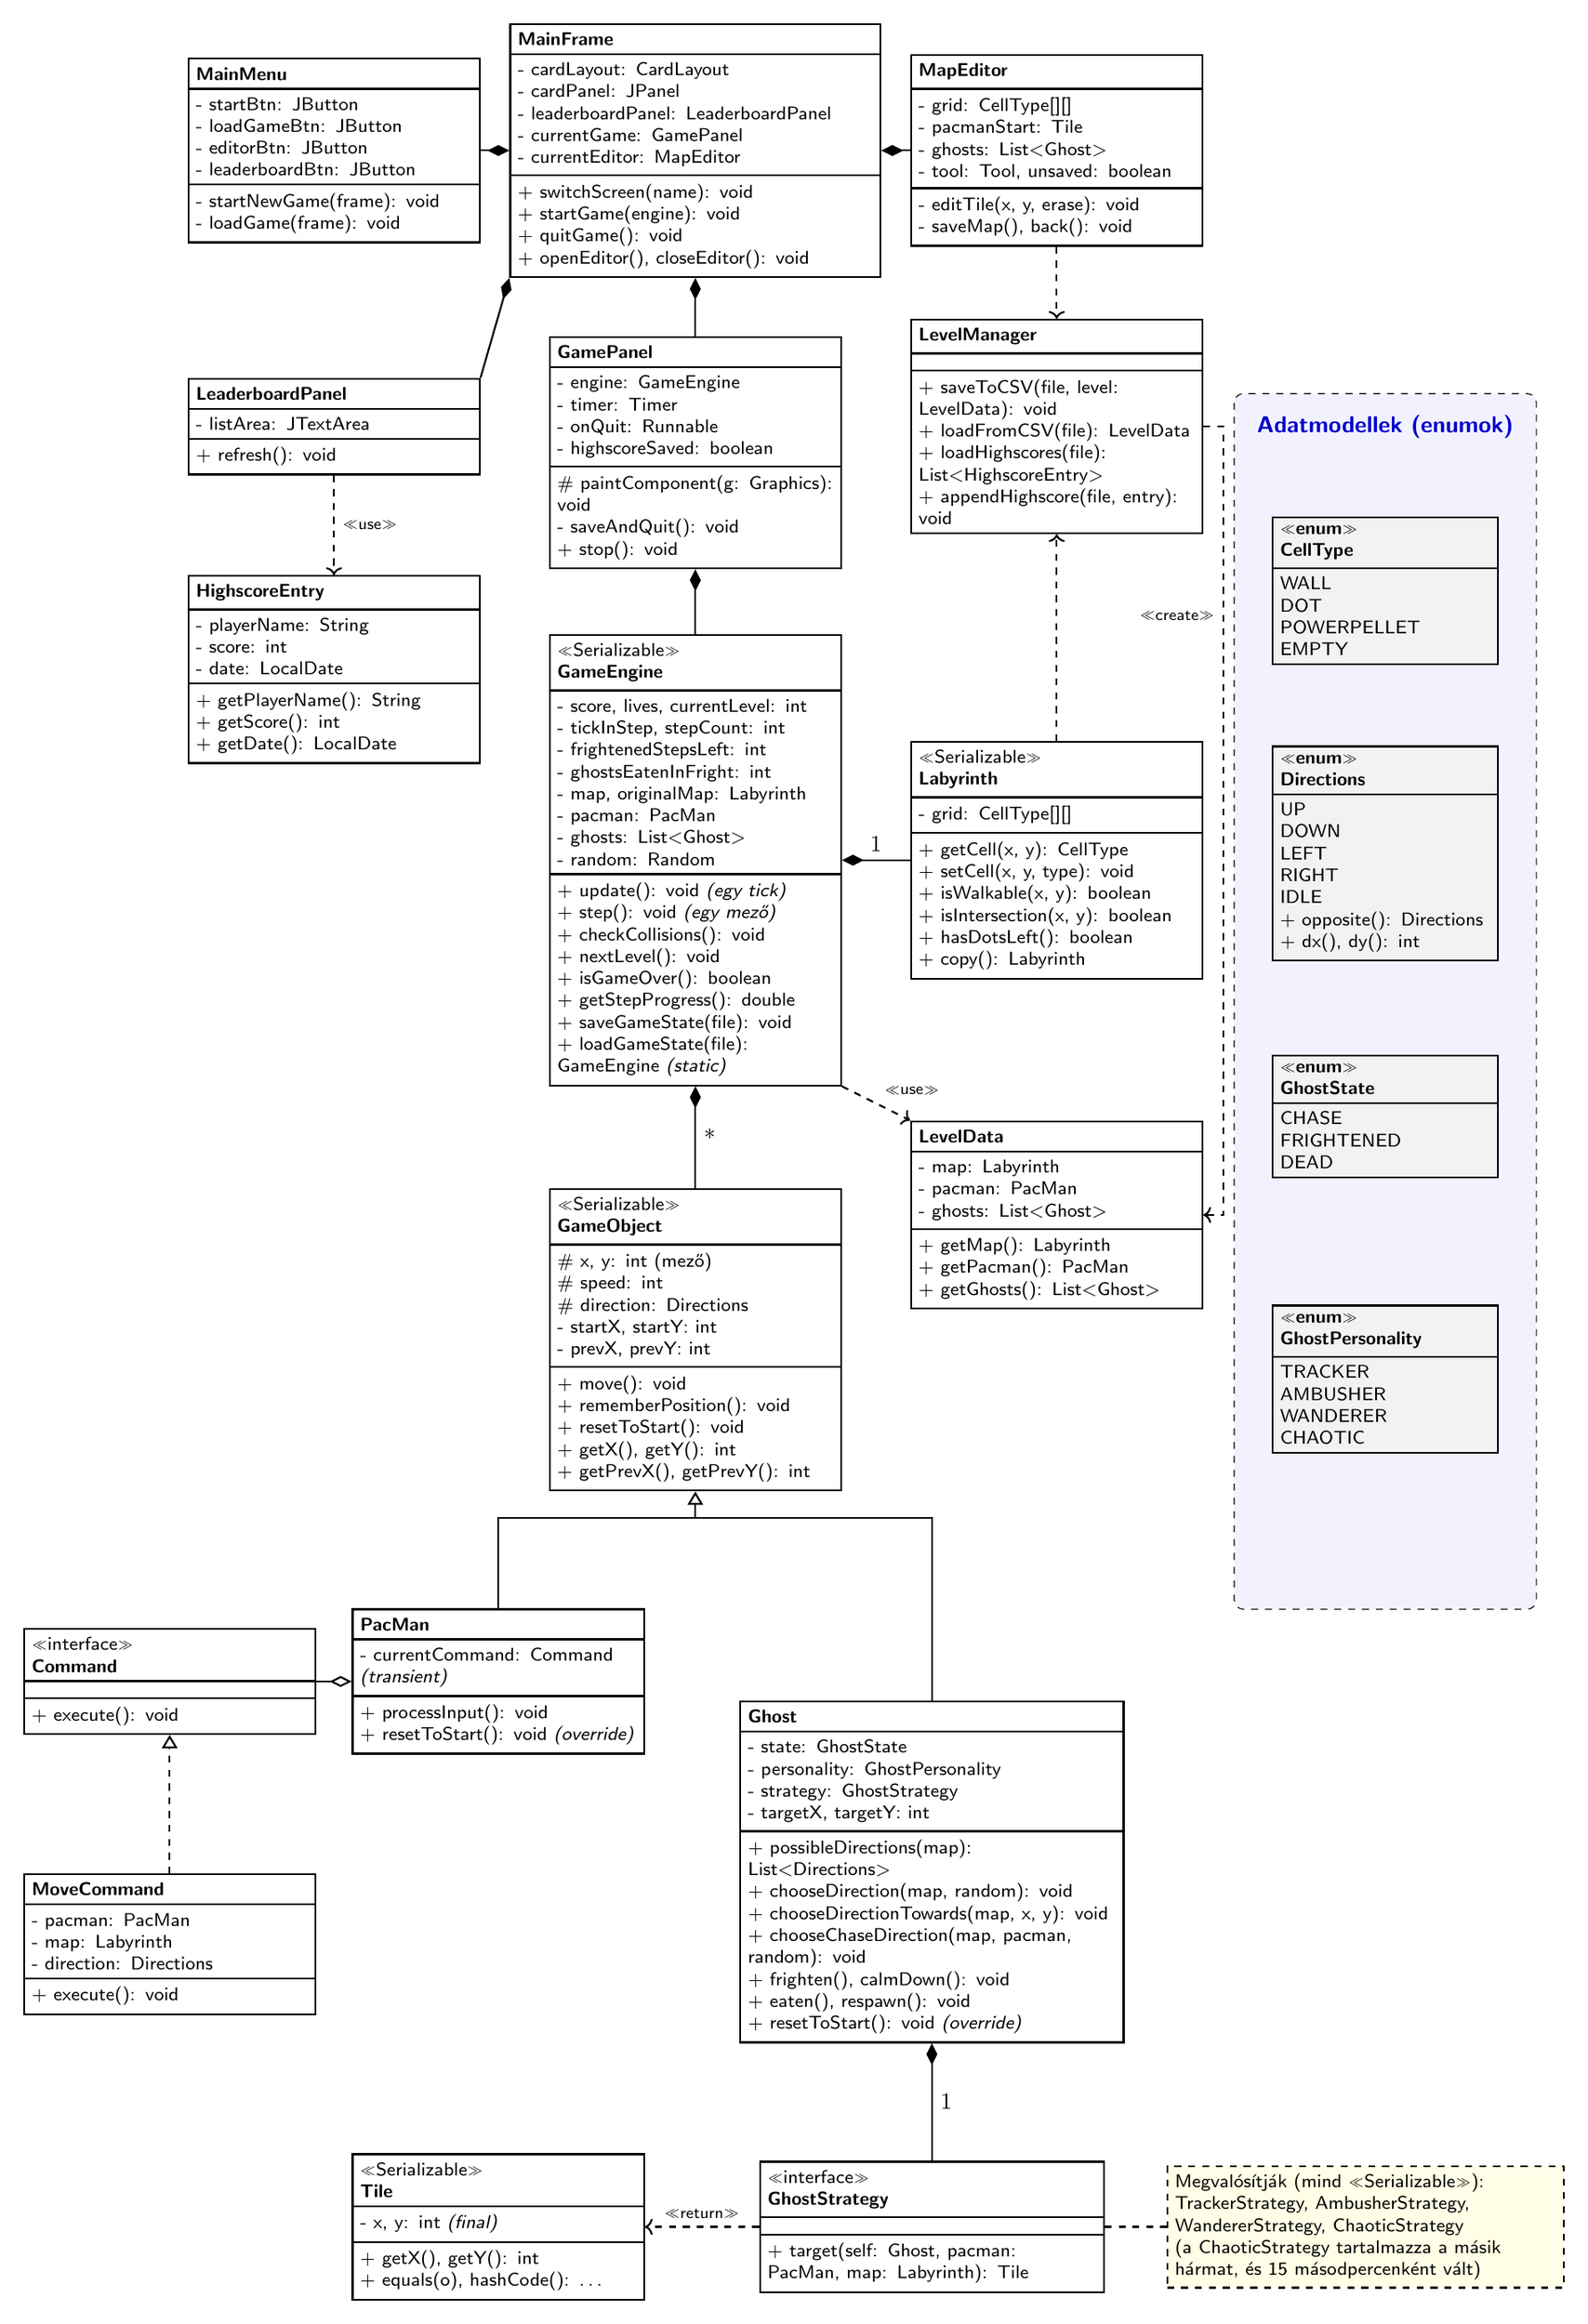
\begin{tikzpicture}[
        umlclass/.style={
            draw, thick,
            rectangle split,
            rectangle split parts=3,
            font=\sffamily\footnotesize, % Olvashatóbb, nagyobb betűméret
            align=left,
            text width=4.2cm,
            fill=white
        },
        umlenum/.style={
            draw, thick,
            rectangle split,
            rectangle split parts=2,
            font=\sffamily\footnotesize,
            align=left,
            text width=3.2cm,
            fill=gray!10
        }
    ]
        
        % === FELHASZNÁLÓI FELÜLET ÉS KEZELŐOSZTÁLYOK ===
        \node[umlclass, text width=5.4cm] (MainFrame) at (0, 8.2) {
            \textbf{MainFrame}
            \nodepart{two}
            - cardLayout: CardLayout \\
            - cardPanel: JPanel \\
            - leaderboardPanel: LeaderboardPanel \\
            - currentGame: GamePanel \\
            - currentEditor: MapEditor
            \nodepart{three}
            + switchScreen(name): void \\
            + startGame(engine): void \\
            + quitGame(): void \\
            + openEditor(), closeEditor(): void
        };

        \node[umlclass] (MainMenu) at (-5.5, 8.2) {
            \textbf{MainMenu}
            \nodepart{two}
            - startBtn: JButton \\
            - loadGameBtn: JButton \\
            - editorBtn: JButton \\
            - leaderboardBtn: JButton
            \nodepart{three}
            - startNewGame(frame): void \\
            - loadGame(frame): void
        };

        \node[umlclass] (LeaderboardPanel) at (-5.5, 4.0) {
            \textbf{LeaderboardPanel}
            \nodepart{two}
            - listArea: JTextArea
            \nodepart{three}
            + refresh(): void
        };

        \node[umlclass] (HighscoreEntry) at (-5.5, 0.3) {
            \textbf{HighscoreEntry}
            \nodepart{two}
            - playerName: String \\
            - score: int \\
            - date: LocalDate
            \nodepart{three}
            + getPlayerName(): String \\
            + getScore(): int \\
            + getDate(): LocalDate
        };

        \node[umlclass] (MapEditor) at (5.5, 8.2) {
            \textbf{MapEditor}
            \nodepart{two}
            - grid: CellType[][] \\
            - pacmanStart: Tile \\
            - ghosts: List$<$Ghost$>$ \\
            - tool: Tool, unsaved: boolean
            \nodepart{three}
            - editTile(x, y, erase): void \\
            - saveMap(), back(): void
        };

        \node[umlclass] (LevelManager) at (5.5, 4.0) {
            \textbf{LevelManager}
            \nodepart{two}
            % Nincs belső állapot (Utility/Factory)
            \nodepart{three}
            + saveToCSV(file, level: LevelData): void \\
            + loadFromCSV(file): LevelData \\
            + loadHighscores(file): List$<$HighscoreEntry$>$ \\
            + appendHighscore(file, entry): void
        };

        \node[umlclass] (GamePanel) at (0, 3.6) {
            \textbf{GamePanel}
            \nodepart{two}
            - engine: GameEngine \\
            - timer: Timer \\
            - onQuit: Runnable \\
            - highscoreSaved: boolean
            \nodepart{three}
            \# paintComponent(g: Graphics): void \\
            - saveAndQuit(): void \\
            + stop(): void
        };


        % === A JÁTÉK MAGJA (MODELL) ===
        \node[umlclass] (GameEngine) at (0, -2.6) {
            \guillemotleft Serializable\guillemotright \\
            \textbf{GameEngine}
            \nodepart{two}
            - score, lives, currentLevel: int \\
            - tickInStep, stepCount: int \\
            - frightenedStepsLeft: int \\
            - ghostsEatenInFright: int \\
            - map, originalMap: Labyrinth \\
            - pacman: PacMan \\
            - ghosts: List$<$Ghost$>$ \\
            - random: Random
            \nodepart{three}
            + update(): void \textit{(egy tick)} \\
            + step(): void \textit{(egy mező)} \\
            + checkCollisions(): void \\
            + nextLevel(): void \\
            + isGameOver(): boolean \\
            + getStepProgress(): double \\
            + saveGameState(file): void \\
            + loadGameState(file): GameEngine \textit{(static)}
        };

        \node[umlclass] (Labyrinth) at (5.5, -2.6) {
            \guillemotleft Serializable\guillemotright \\
            \textbf{Labyrinth}
            \nodepart{two}
            - grid: CellType[][]
            \nodepart{three}
            + getCell(x, y): CellType \\
            + setCell(x, y, type): void \\
            + isWalkable(x, y): boolean \\
            + isIntersection(x, y): boolean \\
            + hasDotsLeft(): boolean \\
            + copy(): Labyrinth
        };

        \node[umlclass] (GameObject) at (0, -9.9) {
            \guillemotleft Serializable\guillemotright \\
            \textbf{\textit{GameObject}}
            \nodepart{two}
            \# x, y: int (mező) \\
            \# speed: int \\
            \# direction: Directions \\
            - startX, startY: int \\
            - prevX, prevY: int
            \nodepart{three}
            + move(): void \\
            + rememberPosition(): void \\
            + resetToStart(): void \\
            + getX(), getY(): int \\
            + getPrevX(), getPrevY(): int
        };

        \node[umlclass] (PacMan) at (-3, -15.1) {
            \textbf{PacMan}
            \nodepart{two}
            - currentCommand: Command \textit{(transient)}
            \nodepart{three}
            + processInput(): void \\
            + resetToStart(): void \textit{(override)}
        };
        
        \node[umlclass] (Command) at (-8, -15.1) {
            \guillemotleft interface\guillemotright \\
            \textbf{Command}
            \nodepart{two}
            \nodepart{three}
            + execute(): void
        };

        \node[umlclass, text width=5.6cm] (Ghost) at (3.6, -18.0) {
            \textbf{Ghost}
            \nodepart{two}
            - state: GhostState \\
            - personality: GhostPersonality \\
            - strategy: GhostStrategy \\
            - targetX, targetY: int
            \nodepart{three}
            + possibleDirections(map): List$<$Directions$>$ \\
            + chooseDirection(map, random): void \\
            + chooseDirectionTowards(map, x, y): void \\
            + chooseChaseDirection(map, pacman, random): void \\
            + frighten(), calmDown(): void \\
            + eaten(), respawn(): void \\
            + resetToStart(): void \textit{(override)}
        };

        \node[umlclass] (MoveCommand) at (-8, -19.1) {
            \textbf{MoveCommand}
            \nodepart{two}
            - pacman: PacMan \\
            - map: Labyrinth \\
            - direction: Directions
            \nodepart{three}
            + execute(): void
        };

        \node[umlclass] (LevelData) at (5.5, -8.0) {
            \textbf{LevelData}
            \nodepart{two}
            - map: Labyrinth \\
            - pacman: PacMan \\
            - ghosts: List$<$Ghost$>$
            \nodepart{three}
            + getMap(): Labyrinth \\
            + getPacman(): PacMan \\
            + getGhosts(): List$<$Ghost$>$
        };

        \node[umlclass, text width=5.0cm] (GhostStrategy) at (3.6, -23.4) {
            \guillemotleft interface\guillemotright \\
            \textbf{GhostStrategy}
            \nodepart{two}
            \nodepart{three}
            + target(self: Ghost, pacman: PacMan, map: Labyrinth): Tile
        };

        \node[umlclass] (Tile) at (-3, -23.4) {
            \guillemotleft Serializable\guillemotright \\
            \textbf{Tile}
            \nodepart{two}
            - x, y: int \textit{(final)}
            \nodepart{three}
            + getX(), getY(): int \\
            + equals(o), hashCode(): \ldots
        };

        \node[draw, dashed, thick, font=\sffamily\footnotesize, align=left, text width=5.8cm, fill=yellow!10] (StrategyNote) at (10.2, -23.4) {
            Megvalósítják (mind \guillemotleft Serializable\guillemotright): \\
            TrackerStrategy, AmbusherStrategy, \\
            WandererStrategy, ChaoticStrategy \\
            (a ChaoticStrategy tartalmazza a másik \\
            hármat, és 15 másodpercenként vált)
        };

        % === ADATMODELLEK (ENUMOK) SZUPERÁLT BLOKK ===
        % Dedikált, halvány hátterű keret az enumoknak
       \draw[dashed, fill=blue!5, rounded corners] (8.2, 4.5) rectangle (12.8, -14.0);
        \node[font=\sffamily\bfseries, text=blue!80!black] at (10.5, 4.0) {Adatmodellek (enumok)};

        \node[umlenum] (CellType) at (10.5, 1.5) {
            \textbf{\guillemotleft enum\guillemotright \\ CellType}
            \nodepart{two}
            WALL \\ DOT \\ POWERPELLET \\ EMPTY
        };

        \node[umlenum] (Directions) at (10.5, -2.5) {
            \textbf{\guillemotleft enum\guillemotright \\ Directions}
            \nodepart{two}
            UP \\ DOWN \\ LEFT \\ RIGHT \\ IDLE \\
            + opposite(): Directions \\
            + dx(), dy(): int
        };

        \node[umlenum] (GhostState) at (10.5, -6.5) {
            \textbf{\guillemotleft enum\guillemotright \\ GhostState}
            \nodepart{two}
            CHASE \\ FRIGHTENED \\ DEAD
        };

        \node[umlenum] (GhostPersonality) at (10.5, -10.5) {
            \textbf{\guillemotleft enum\guillemotright \\ GhostPersonality}
            \nodepart{two}
            TRACKER \\ AMBUSHER \\ WANDERER \\ CHAOTIC
        };

        % === KAPCSOLATOK ===
        % UI dependenciák és kompozíciók
        \draw[{Diamond[fill=black, scale=1.2]}-, thick] (MainFrame.west) -- (MainMenu.east);
        \draw[{Diamond[fill=black, scale=1.2]}-, thick] (MainFrame.east) -- (MapEditor.west);
        \draw[{Diamond[fill=black, scale=1.2]}-, thick] (MainFrame.south) -- (GamePanel.north);
        \draw[{Diamond[fill=black, scale=1.2]}-, thick] (MainFrame.south west) -- (LeaderboardPanel.north east);
        \draw[dashed, ->, thick] (LeaderboardPanel.south) -- (HighscoreEntry.north) node[midway, right, font=\sffamily\scriptsize] {\guillemotleft use\guillemotright};
        
        \draw[dashed, ->, thick] (MapEditor.south) -- (LevelManager.north);
        \draw[dashed, ->, thick] (Labyrinth.north) -- (LevelManager.south);
        \draw[{Diamond[fill=black, scale=1.2]}-, thick] (GamePanel.south) -- (GameEngine.north);

        % Modell kapcsolatok
        \draw[{Diamond[fill=black, scale=1.2]}-, thick] (GameEngine.east) -- (Labyrinth.west) node[midway, above] {1};
        \draw[{Diamond[fill=black, scale=1.2]}-, thick] (GameEngine.south) -- (GameObject.north) node[midway, right] {*};

        % Öröklődés
        \draw[-{Triangle[open, fill=white, scale=1.2]}, thick] ([yshift=-0.4cm]GameObject.south) -- (GameObject.south);
        \draw[thick] (PacMan.north) |- ([yshift=-0.4cm]GameObject.south);
        \draw[thick] (Ghost.north) |- ([yshift=-0.4cm]GameObject.south);
        
        % Command minta: aggregáció
        \draw[{Diamond[fill=white, scale=1.2]}-, thick] (PacMan.west) -- (Command.east);
        % A MoveCommand megvalósítja a Command interfészt
        \draw[dashed, -{Triangle[open, fill=white, scale=1.2]}, thick] (MoveCommand.north) -- (Command.south);

        % LevelData: a LevelManager hozza létre, a GameEngine ebből épül fel
        \draw[dashed, ->, thick] (LevelManager.east) -- ++(0.3, 0) |- (LevelData.east) node[pos=0.12, left, font=\sffamily\scriptsize] {\guillemotleft create\guillemotright};
        \draw[dashed, ->, thick] (GameEngine.south east) -- (LevelData.north west) node[midway, above right, font=\sffamily\scriptsize] {\guillemotleft use\guillemotright};

        % Strategy minta: a szellem birtokolja a stratégiaobjektumát
        \draw[{Diamond[fill=black, scale=1.2]}-, thick] (Ghost.south) -- (GhostStrategy.north) node[midway, right] {1};
        \draw[dashed, thick] (GhostStrategy.east) -- (StrategyNote.west);
        \draw[dashed, ->, thick] (GhostStrategy.west) -- (Tile.east) node[midway, above, font=\sffamily\scriptsize] {\guillemotleft return\guillemotright};

    \end{tikzpicture}
    } % \resizebox vége
    \caption{A teljes játékarchitektúra UML osztálydiagramja}
    \label{fig:uml_complete_diagram}
\end{figure}

% --- 4. Játékciklus ---
\section{Játékciklus, mozgás és ütközések}
\label{sec:game_loop}
\begin{itemize}[itemsep=2pt]
    \item \textbf{Tick és lépés:} a \texttt{GamePanel} \texttt{Timer}-e $1000/60 \approx 16$~ms-onként meghívja az \texttt{engine.update()}-et, majd a \texttt{repaint()}-et. Minden 10. tick (\texttt{TICKS\_PER\_STEP}) egy \texttt{step()}, amely minden szereplőt legfeljebb egy mezővel mozgat: 6 mező/másodperc. Minden játékszabály a \texttt{step()}-ben fut, ezért a tesztek közvetlenül azt hívják.
    \item \textbf{Folyamatos rajzolás:} a \texttt{getStepProgress()} ($0.0$--$1.0$) megadja, hol tart a lépés, és a nézet minden szereplőt az $(\textit{előző} + (\textit{aktuális} - \textit{előző}) \cdot \textit{haladás}) \cdot \textit{TILE}$ pixelpozícióra rajzol. A modell csak egész mezőket ismer.
    \item \textbf{Szálkezelés:} a \texttt{Timer} eseménye és a billentyűzet is az Event Dispatch Thread szálon fut, így a modellt egyszerre csak egy szál éri el, külön szinkronizáció nélkül.
\end{itemize}

\textbf{Egy lépés sorrendje:}
\begin{enumerate}[itemsep=1pt]
    \item Ha vége a játéknak, nem történik semmi.
    \item Fogy az ijedtség-időzítő; ha lejár, minden szellem \texttt{calmDown()}-t kap.
    \item Pac-Man végrehajtja a pufferelt parancsát, és lép, ha nincs előtte fal.
    \item Minden szellem az állapota szerint választ irányt és lép: \texttt{DEAD} -- haza, a kezdőmezőjére; \texttt{FRIGHTENED} -- véletlenszerűen, és csak minden 2. lépésben (fél sebesség); \texttt{CHASE} -- a stratégiája célmezője felé. Lépés után a \texttt{respawn()} a hazaért \texttt{DEAD} szellemet \texttt{CHASE}-re állítja.
    \item Ütközésvizsgálat (\texttt{checkCollisions()}), miután már mindenki lépett.
    \item Ha nem maradt pötty és power pellet: \texttt{nextLevel()}.
\end{enumerate}
Mozgás előtt mindenki elmenti az előző mezőjét (\texttt{rememberPosition()}), akkor is, ha áll.

\textbf{A szellemek útvonalválasztása:} a szellem sosem fordul vissza 180 fokban, kivéve zsákutcában és az ijedtség kezdetén. Folyosóban csak egy irány marad, így valódi döntés csak kereszteződésben történik. A \texttt{chooseDirectionTowards} azt a lehetséges irányt választja, amelynek a következő mezője a célmezőhöz a legközelebb van ($dx^2 + dy^2$, gyökvonás nélkül; egyenlőségnél az \texttt{UP}, \texttt{DOWN}, \texttt{LEFT}, \texttt{RIGHT} sorrend dönt). Ez mohó választás: kiszámítható, de nem mindig a legrövidebb út.

\textbf{Ütközések és pontozás:}
\begin{itemize}[itemsep=2pt]
    \item \textbf{Pötty} 10, \textbf{power pellet} 50 pont; a mező \texttt{EMPTY} lesz. A pellet minden szellemen \texttt{frighten()}-t hív, újraindítja az ijedtség-időzítőt, és nullázza a szellemevési sorozatot.
    \item \textbf{Találkozás:} Pac-Man és egy szellem akkor találkozik, ha a lépés után ugyanazon a mezőn állnak, \textit{vagy} helyet cseréltek (különben átmennének egymáson).
    \item \textbf{Két menet,} hogy a szellemek sorrendje ne számítson: előbb minden ütköző ijedt szellemet megeszik (\texttt{DEAD} lesz; egy ijedtségen belül 200, 400, 800, 1600 pont, azaz $200 \cdot 2^n$, legfeljebb 1600), utána bármely ütköző, nem \texttt{DEAD} szellem megöli Pac-Mant.
    \item \textbf{Életvesztés:} egy élet (lépésenként legfeljebb egy), Pac-Man és minden szellem visszakerül a kezdőmezőjére \texttt{CHASE} állapotban, az ijedtség megszűnik; a megevett pöttyök nem jönnek vissza. Az \texttt{isGameOver()} az életekből számolódik (\texttt{lives <= 0}).
    \item \textbf{Az ijedtség hossza} szintenként csökken (a sebességek nem változnak):
\end{itemize}
\begin{center}
\begin{tabular}{@{}lcccc@{}}
    \toprule
    \textbf{Szint} & 1--3 & 4--6 & 7--10 & 11+ \\
    \midrule
    \textbf{Másodperc (lépés)} & 6 (36) & 4 (24) & 2 (12) & 1 (6) \\
    \bottomrule
\end{tabular}
\end{center}

% --- 5. Tervezési minták ---
\section{Tervezési minták}
\label{sec:design_patterns}
\begin{itemize}[itemsep=3pt]
    \item \textbf{Strategy (a szellemek célmezője):} minden személyiség célmezője külön osztály, amely a \texttt{GhostStrategy} interfész \texttt{Tile target(Ghost self, PacMan pacman, Labyrinth map)} metódusát valósítja meg. A \texttt{Ghost} adattagként tárolja a stratégiáját (kompozíció öröklés helyett), és a konstruktorban a személyisége alapján kapja meg. A stratégia csak azt mondja meg, \textit{hová} menjen a szellem, azt, hogy \textit{merre} lépjen, a \texttt{chooseDirectionTowards} dönti el.
    \begin{itemize}[itemsep=1pt]
        \item \textbf{TRACKER} (piros, \texttt{TrackerStrategy}): Pac-Man mezője.
        \item \textbf{AMBUSHER} (rózsaszín, \texttt{AmbusherStrategy}): 4 mezővel Pac-Man előtt, az iránya szerint (\texttt{Directions.dx()}, \texttt{dy()}).
        \item \textbf{WANDERER} (narancs, \texttt{WandererStrategy}): Pac-Man mezője, de ha legfeljebb 8 mezőre van tőle ($dx^2 + dy^2 \le 64$), a saját kezdőmezője a szellemházban; amint újra messzebb van, ismét üldöz.
        \item \textbf{CHAOTIC} (cián, \texttt{ChaoticStrategy}): a másik hármat tartalmazza, és 90 lépésenként (15~s üldözés) véletlenszerűen vált közöttük. Ez indokolja a mintát: egy objektum futás közben nem cserélheti az osztályát, de a stratégiaobjektumát igen.
    \end{itemize}
    \item \textbf{Véges állapotgép (\texttt{GhostState}: \texttt{CHASE}, \texttt{FRIGHTENED}, \texttt{DEAD}):} minden átmenetnek saját metódusa van, amely maga ellenőrzi a feltételét, így rossz állapotban hívva nem csinál semmit (\ref{fig:ghost_fsm}.~ábra):

    \vspace{0.1cm}
    \begin{tabular}{@{}lll@{}}
        \toprule
        \textbf{Esemény} & \textbf{Metódus} & \textbf{Melyik állapotból} \\
        \midrule
        Power pellet & \texttt{frighten()} & bármelyikből, kivéve \texttt{DEAD} (először megfordul) \\
        Lejár az ijedtség & \texttt{calmDown()} & csak \texttt{FRIGHTENED} \\
        Pac-Man megeszi & \texttt{eaten()} & csak \texttt{FRIGHTENED} \\
        Hazaér & \texttt{respawn()} & \texttt{DEAD}, a kezdőmezőjén \\
        \bottomrule
    \end{tabular}
    \vspace{0.1cm}

    Az ijedt szellem fehér, a \texttt{DEAD} szellem csak egy kis szürke pont (a szeme), és ártalmatlan. Életvesztéskor a \texttt{resetToStart()} mindenkit \texttt{CHASE}-re állít; ez újraindítás, nem az ábra éle.
    \item \textbf{Command és bemenetpufferelés:} a \texttt{GamePanel} minden WASD lenyomásra egy \texttt{MoveCommand}-ot ad Pac-Mannek, amely a következő lépésekben fut le: ha a kívánt irányban szabad az út, Pac-Man elfordul, ha nem, a parancs megmarad, és a következő lépésben újra próbálkozik. Így a korán lenyomott kanyar az első lehetséges mezőn megtörténik.
    \item \textbf{Factory:} a \texttt{LevelManager} egy pályafájlból felépíti a labirintust és a szereplőket, és egy \texttt{LevelData}-ban adja vissza; a motor nem ismeri a fájlformátumot.
    \item \textbf{A nézet frissítése:} a motor nem értesít senkit, nincsenek figyelői. A \texttt{GamePanel} \texttt{Timer}-e minden tickben meghívja az \texttt{update()}-et, majd a \texttt{repaint()}-et, és a \texttt{paintComponent} a getterekből olvas. A függőség csak a nézettől a modell felé mutat.
\end{itemize}

\begin{figure}[ht]
    \centering
    \resizebox{0.55\textwidth}{!}{ % Felnagyítja az ábrát a lapszélesség 90%-ára
    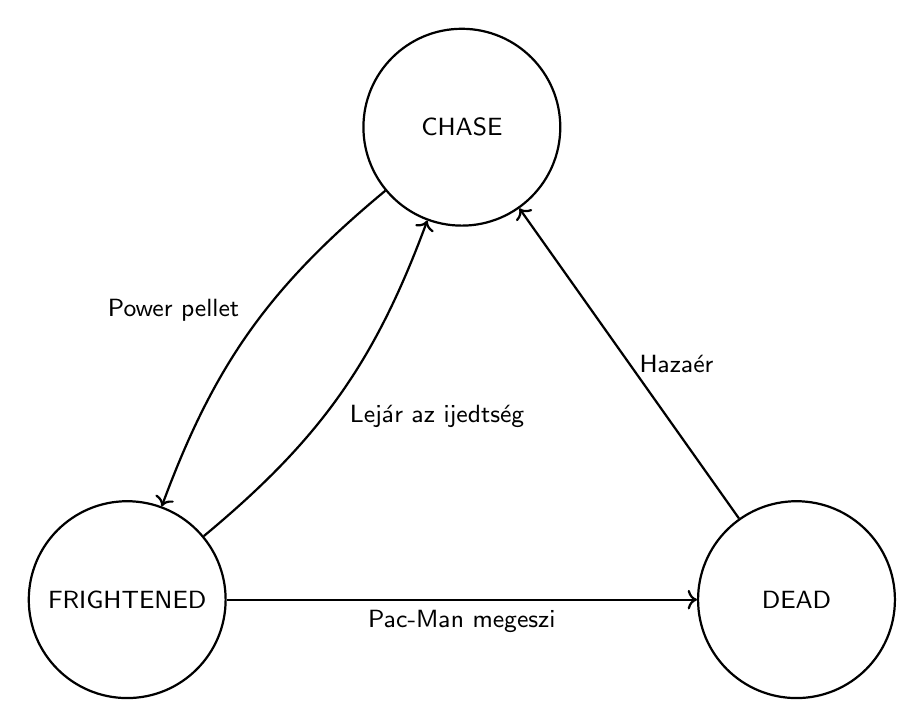
\begin{tikzpicture}[->, auto, thick,
                        every node/.style={font=\sffamily\small},
                        state/.style={draw, circle, minimum size=2.5cm, align=center}]
        
        % Az állapotok kézzel elhelyezve, a legjobb kompatibilitásért
        \node[state] (Chase) at (4.25, 0) {CHASE};
        \node[state] (Frightened) at (0, -6) {FRIGHTENED};
        \node[state] (Dead) at (8.5, -6) {DEAD};

        \path
        (Chase) edge [bend right=15] node [above left] {Power pellet} (Frightened)
        (Frightened) edge [bend right=15] node [below right] {Lejár az ijedtség} (Chase)
        (Frightened) edge node [below] {Pac-Man megeszi} (Dead)
        (Dead) edge node [right] {Hazaér} (Chase);
    \end{tikzpicture}
    } % \resizebox vége
    \caption{A szellemek viselkedésének véges állapotgépe (FSM)}
    \label{fig:ghost_fsm}
\end{figure}

% --- 6. Fájlkezelés ---
\section{Fájlkezelés és perzisztencia}
\label{sec:io}
Minden útvonal a munkakönyvtárhoz képest relatív, ezért a játékot a projekt mappájából kell indítani.
\begin{itemize}[itemsep=3pt]
    \item \textbf{Ranglista -- \texttt{highscores.csv}:} soronként \texttt{PlayerName;Score;Date}, például \texttt{balazs;2350;2026-11-09}. Az \texttt{appendHighscore} beolvassa a sorokat, hozzáadja az újat, pontszám szerint csökkenően rendezi, és újraírja a fájlt. A hiányzó fájl üres ranglista; a hibás sort a program a sorszámával együtt elutasítja (\texttt{IllegalArgumentException}).
    \item \textbf{Játékállás -- \texttt{saves/*.dat}:} a teljes \texttt{GameEngine} \texttt{ObjectOutputStream}-mel, binárisan; betöltés \texttt{ObjectInputStream}-mel. Ehhez minden modellosztály (és a stratégiák) \texttt{Serializable}. A \texttt{currentCommand} \texttt{transient}, mert a pufferelt billentyű bemenet, nem állapot. Ha a fájl nem \texttt{GameEngine}-t tartalmaz, \texttt{IOException} keletkezik, és a menü hibaüzenetet mutat. A modellosztályok nem deklarálnak \texttt{serialVersionUID}-t, ezért egy osztály megváltozása után a régi mentések nem tölthetők be.
    \item \textbf{Pályák -- \texttt{maps/*.txt}:} a labirintus karakteres rajza, soronként egy pályasor, mezőnként egy karakter. Minden sornak azonos hosszúnak kell lennie, pontosan egy \texttt{P} kell; ismeretlen karakter esetén hibát jelez a sor és oszlop megadásával. A szereplők jelei alatt \texttt{EMPTY} mező van, a szellemek kezdőmezői jelölik ki a szellemházat.
\end{itemize}

\begin{center}
\begin{tabular}{@{}cl@{\hspace{1.5cm}}cl@{}}
    \toprule
    \textbf{Jel} & \textbf{Jelentés} & \textbf{Jel} & \textbf{Jelentés} \\
    \midrule
    \texttt{\#} & fal (\texttt{WALL}) & \texttt{P} & Pac-Man kezdőmezője \\
    \texttt{.} & pötty (\texttt{DOT}) & \texttt{T} / \texttt{A} & \texttt{TRACKER} / \texttt{AMBUSHER} szellem \\
    \texttt{o} & power pellet & \texttt{W} / \texttt{C} & \texttt{WANDERER} / \texttt{CHAOTIC} szellem \\
    \texttt{\_} & üres padló (\texttt{EMPTY}) & & \\
    \bottomrule
\end{tabular}
\qquad
\begin{minipage}{3cm}
\begin{verbatim}
#########
#P..o...#
#.##_##.#
#..T_A..#
#########
\end{verbatim}
\end{minipage}
\end{center}

% --- 7. Tesztek ---
\section{Egységtesztelés}
16 JUnit 5 teszt, 4 tesztosztályban, a tesztelt osztállyal azonos csomagban. Csak a modellt és a fájlkezelést tesztelik, Swing nélkül. Minden osztály \texttt{@BeforeEach} fixture-rel indul, a tesztek Arrange--Act--Assert szerkezetűek, a \texttt{step()}-et hívják az \texttt{update()} helyett, és rögzített seedű \texttt{Random}-ot használnak.

\vspace{0.1cm}
\begin{tabular}{@{}p{3.4cm}p{12.0cm}@{}}
    \toprule
    \textbf{Tesztosztály} & \textbf{Mit ellenőriz} \\
    \midrule
    \texttt{GameEngineTest} (10) & falnak ütközés; pötty megevése; a blokkolt kanyar nem állítja meg a lépést; kereszteződés felismerése; power pellet: pont és \texttt{FRIGHTENED}; halál: életvesztés és visszaállás; ijedt szellem megevése; Game Over; az Ambusher célmezője; \texttt{nextLevel()} \\
    \texttt{GhostTest} (2) & \texttt{respawn()}: távol \texttt{DEAD} marad, otthon \texttt{CHASE} lesz \\
    \texttt{LabyrinthTest} (2) & \texttt{hasDotsLeft()}: igaz, amíg marad power pellet; hamis, ha minden elfogyott \\
    \texttt{LevelManagerTest} (2) & hiányzó fájl: \texttt{IOException}; ismeretlen jel: \texttt{IllegalArgumentException} (\texttt{assertThrows}, \texttt{@TempDir}) \\
    \bottomrule
\end{tabular}
\newpage
% --- 8. Kézikönyv ---
\section{Felhasználói kézikönyv}
\textbf{Indítás} (Java 17+, a projekt mappájából): \texttt{mvn compile}, majd \texttt{java -cp target/classes hu.bme.pacman.system.Main}.

\begin{itemize}[itemsep=2pt]
    \item \textbf{Főmenü:} \textit{Start new game} (pályaválasztás), \textit{Load previous game} (mentés betöltése), \textit{Leaderboard}, \textit{Create map}.
    \item \textbf{Játék:} \texttt{W} fel, \texttt{A} balra, \texttt{S} le, \texttt{D} jobbra. Pac-Man addig halad, amíg falhoz nem ér; a kanyar előre is lenyomható. Pontok: pötty 10, power pellet 50, szellemek 200/400/800/1600. Power pellet után a szellemek fehérek, fele sebességgel kóborolnak, és megehetők; a megevett szellem szeme hazasiet. A színes szellem érintése egy életbe kerül.
    \item \textbf{Mentés:} \textit{SAVE \& QUIT} vagy \texttt{F5}; a \texttt{saves} mappába tetszőleges névvel menthet (a \texttt{.dat} kiterjesztést a program hozzáteszi, felülírás előtt rákérdez). Megszakításkor vagy hibánál a játék folytatódik. \texttt{GAME OVER} után a gomb mentés nélkül lép vissza a menübe.
    \item \textbf{Pályaszerkesztő:} válasszon eszközt jobb oldalt, rajzoljon bal egérgombbal, töröljön jobbal (húzással is). Pac-Man kezdőmezőjéből csak egy lehet. A \textit{SAVE MAP} csak Pac-Mannel és legalább egy pöttyel ment; a \textit{BACK} mentetlen változásnál rákérdez. Hagyjon utat minden pöttyhöz és a szellemház nyílásaihoz.
    \item \textbf{Ismert korlát:} az ablak bezárása azonnal kilép, és nem kérdez rá a mentetlen játékra vagy pályára.
\end{itemize}

\end{document}
